\chapter{模型介绍}
\label{chapter:model}
\section{SARIMA模型}

SARIMA(季节性自回归积分滑动平均)模型是时间序列分析中的经典方法,广泛应用于具有周期性和趋势性的时间序列建模任务。该模型在ARIMA模型的基础上引入了季节性成分,使其能够有效捕捉周期性波动,弥补传统ARIMA在处理季节性特征上的不足。总体流程如图\ref{fig:SARIMA模型流程图}所示。

\begin{figure}[H]
    \centering
    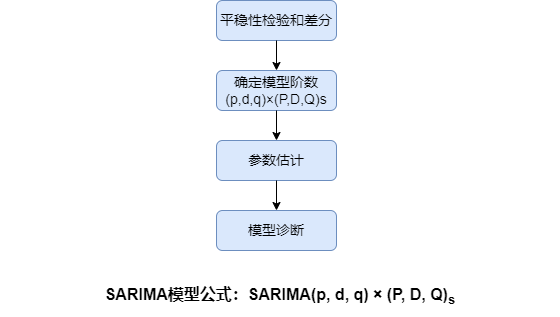
\includegraphics[width=0.75\linewidth]{figure/SARIMA_formula.png}
    \caption{SARIMA模型流程图}
    \label{fig:SARIMA模型流程图}
\end{figure}

其数学表达式可以表示为:

\[
\Phi_P(B^s) \, \phi_p(B) \, (1-B)^d \, (1-B^s)^D \, X_t \;=\; \Theta_Q(B^s) \, \theta_q(B) \, \varepsilon_t,
\]

其中,\( B \) 表示滞后算子,\( s \) 为周期长度,\( d \) 和 \( D \) 分别代表非季节性和季节性差分次数,用以消除时间序列中的趋势和季节性成分;\( \phi_p(B) \) 与 \( \Phi_P(B^s) \) 分别为非季节性及季节性自回归系数多项式;\( \theta_q(B) \) 与 \( \Theta_Q(B^s) \) 分别为非季节性及季节性移动平均系数多项式;\( \varepsilon_t \) 表示白噪声序列。

SARIMA模型的核心在于利用差分运算去除原始序列中的趋势和季节性成分,再辅以自回归和移动平均结构对去趋势后的数据进行建模,从而实现对具有明显季节性模式的数据进行精准预测. 然而,虽然SARIMA模型在捕捉季节性规律方面具有较强优势,但其在对非线性和复杂模式数据的建模能力上存在局限,因此在面对非线性特征较为显著的时间序列时,可考虑结合其他非线性模型或深度学习方法以提升预测效果。

在实际应用过程中,参数选择尤为关键,通常首先利用自相关函数(ACF)及偏自相关函数(PACF)图进行初步参数估计,随后再通过网格搜索等优化技术,结合信息准则(如AIC、BIC)对模型进行进一步调整和确认.

\section{LSTM模型}

LSTM(长短时记忆网络)模型是深度学习领域中专为时间序列数据建模而设计的一种递归神经网络(RNN)。相比于传统RNN,LSTM通过引入记忆单元(Cell State)和三个门控机制(遗忘门、输入门和输出门),有效缓解了长时间依赖问题中常见的梯度消失或梯度爆炸问题,从而更好地捕捉数据中的非线性关系。其模型结构图如图\ref{fig:LSTM模型结构图}所示。

\begin{figure}[H]
    \centering
    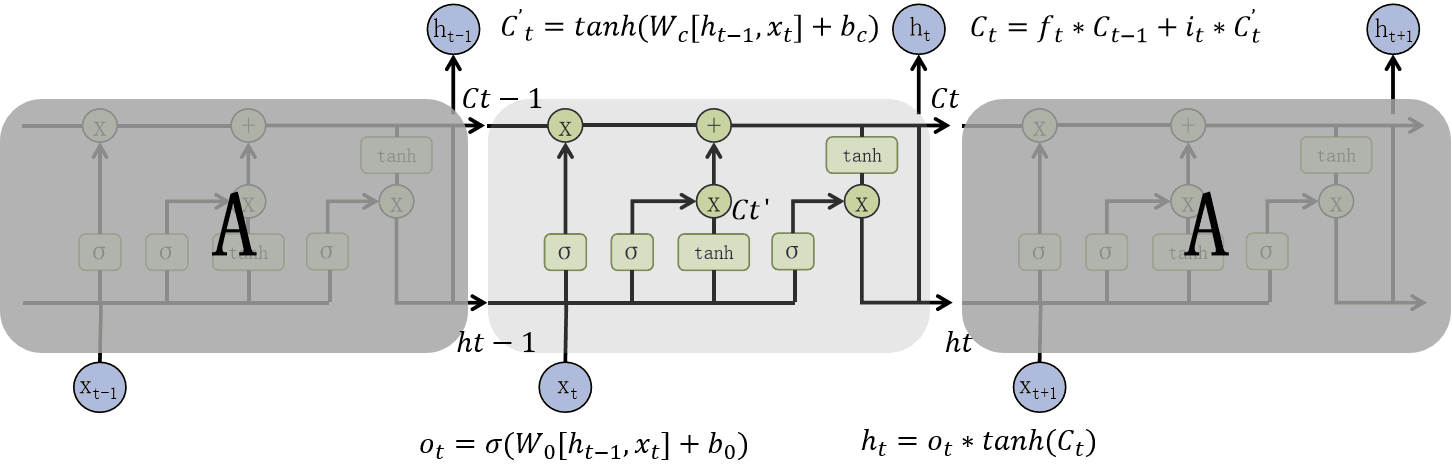
\includegraphics[width=1\linewidth]{figure/LSTM模型结构图.png}
    \caption{LSTM模型结构图}
    \label{fig:LSTM模型结构图}
\end{figure}

其工作机制可以概述如下:

首先,遗忘门决定了哪些历史信息需要被遗忘,其数学表达式为:
\[
f_t = \sigma\Big(W_f\big[h_{t-1},\,x_t\big] + b_f\Big).
\]

其次,输入门负责选择性地更新当前时间步的信息,同时生成候选记忆单元状态:
\[
i_t = \sigma\Big(W_i\big[h_{t-1},\,x_t\big] + b_i\Big), \quad 
C'_t = \tanh\Big(W_C\big[h_{t-1},\,x_t\big] + b_C\Big).
\]

然后,通过结合遗忘门和输入门的输出,更新记忆单元状态:
\[
C_t = f_t \ast C_{t-1} + i_t \ast C'_t.
\]

最后,输出门决定了当前时间步的隐藏状态,其计算过程如下:
\[
o_t = \sigma\Big(W_o\big[h_{t-1},\,x_t\big] + b_o\Big), \quad 
h_t = o_t \ast \tanh(C_t).
\]

LSTM模型因其强大的非线性建模能力,已被广泛应用于金融市场预测、流量预测、气象数据分析等任务。特别地,LSTM的引入有效解决了SARIMA模型在处理非线性问题上的不足,使其在捕捉复杂时间序列中的趋势反转和波动性变化方面表现出色。

总之,LSTM不仅在理论上为序列建模提供了有力的支持,而且在实际应用中,凭借其对非线性特征的高效捕捉能力,为解决SARIMA模型非线性局限性提供了重要补充。

\section{SARIMA-LSTM残差堆叠模型}

SARIMA-LSTM残差堆叠模型\cite{dubey2021study}是一种集成方法,通过组合传统的SARIMA模型和深度学习中的LSTM模型,实现对时间序列数据中线性及非线性成分的联合建模。其模型流程图如\ref{fig:SARIMA_LSTM残差堆叠模型流程图}所示。

\begin{figure}[H]
    \centering
    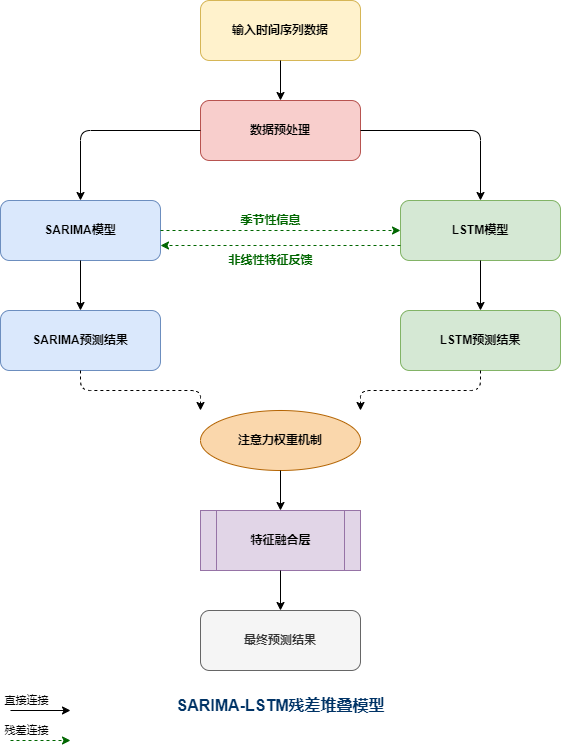
\includegraphics[width=0.6\linewidth]{figure/SARIMA_LSTM.png}
    \caption{SARIMA-LSTM残差堆叠模型流程图}
    \label{fig:SARIMA_LSTM残差堆叠模型流程图}
\end{figure}

首先,利用SARIMA模型对序列中的趋势、季节性以及其他线性模式进行捕捉,从而获得线性部分的预测值。设原始序列为 \(X_t\),经过SARIMA模型预测得到的线性部分为 \(\hat{X}_t^{\text{SARIMA}}\),残差部分可定义为
\[
e_t = X_t - \hat{X}_t^{\text{SARIMA}}.
\]
由于SARIMA模型在处理非线性和复杂动态特征上存在一定局限性,因此采用LSTM模型对预测残差进行建模,挖掘数据中潜在的非线性信息。LSTM模型通过其记忆单元及门控机制,能够捕捉长距离依赖关系和瞬时变化,从而对残差序列进行有效预测,得到 \(\hat{e}_t\)。

最终,模型将SARIMA的预测结果与LSTM对残差的预测结果相结合,形成最终的预测值:
\[
\hat{X}_t = \hat{X}_t^{\text{SARIMA}} + \hat{e}_t.
\]


这种残差堆叠方法既保留了SARIMA在捕捉长期趋势与周期性变化方面的优势,又利用LSTM弥补了对非线性和局部复杂模式的建模不足,从而提升整体预测精度。模型训练过程中,通常先对SARIMA模型进行参数估计和拟合,在确定线性部分后,再对LSTM网络进行残差序列的训练优化,确保两部分模型各自发挥专长。模型预测时,可先用SARIMA获得初步预测,再计算生成残差序列,并将其输入LSTM进行调整和修正,最后输出融合后的预测结果。